\documentclass{article}

\usepackage[margin=0.5in]{geometry}
\usepackage{amsmath}
\usepackage{mathtools}
\usepackage{amssymb}
\usepackage{graphicx}

\author{Craig Ching\\
      \texttt{\#1452647} \\
      \texttt{chin0007@umn.edu}}
\title{
CSCI 5521 Spring 2017 Homework \#4}
\begin{document}

\maketitle

\newcommand{\mysum} {\sum\limits_{i = 1}^n}
\newcommand{\myz} {\mathbf{w}^T x_i}

%\setlength{\parindent}{0pt}

\section{Problem 1}

%1a
\subsection{(a) Professor HighLowHigh claims: $\mathbf{v}^t = \mathbf{x}^t \enspace \text{for all} \enspace t = 1, \dots, N$.  Is the claim correct?}

Given:

\begin{equation}
\begin{aligned}
\mathbf{z}^t &= W^T\mathbf{x}^t \\
\mathbf{v}^t &= W\mathbf{z}^t
\end{aligned}
\end{equation}

The matrix $W$ is the projection matrix and $W \in \mathbb{R}^{D \times d}, d < D$, the first equation is the projection from the original space to a new subspace and the second equation is the projection from the subspace back to the original space.  We can write this transformation combined as:

\begin{equation}
\mathbf{v}^t = WW^T\mathbf{x}^t
\end{equation}

So the claim that $\mathbf{x}^t = \mathbf{v}^t$ can only be true if $WW^T = I$, the identity matrix.  In order for this to be true, $W$ has to be an orthogonal, square matrix, in other words, $W \in \mathbb{R}^{D \times D}$ and then $W^T = W^{-1}$.  But the problem states that $W \in \mathbb{R}^{D \times d}, d < D$, so $W$ can't be orthogonal since it isn't square and $WW^T \neq I$, therefore:

\begin{equation}
\mathbf{v}^t \neq \mathbf{x}^t
\end{equation}


%If we assume that $WW^T$ is the identity matrix, then $W$ must be an orthogonal matrix.  Since W is defined as the PCA projection matrix, it's columns are the eigenvectors of the covariance matrix $\Sigma$.  In order for $W$ to be an orthogonal matrix, all eigenvalues of $\Sigma$ have to be distinct and greater than 0.  So $\mathbf{v}^t = \mathbf{x}^t$ when:


% 1b
\subsection{(b) Professor HighLowHigh also claims: $\sum\limits_{t=1}^N || \mathbf{x}^t ||_2^2 - \sum\limits_{t=1}^N || \mathbf{v}^t ||_2^2 = \sum\limits_{t=1}^N || \mathbf{x}^t - \mathbf{v}^t ||_2^2$.   Is the claim correct?}

I believe this claim is correct.  PCA is an orthogonal transformation of the data potentially to a lower dimension, though not necessarily so.  If the $W$ matrix is formed from all $D$ covariance matrix eigenvalues and all the eigenvalues are distinct, then the transformation $WW^T$ is the identity matrix and:

\begin{equation}
\mathbf{x}^t = \mathbf{v^t}
\end{equation}

and the claim is trivially true.  It is interesting to note that as $d = D, d = D-1, ... d = D-D$, the matrix $WW^T$ starts as the identity matrix $\mathbb{I}$ and each subsequent projection to a lower dimensional space reduces the approximation of the matrix  $WW^T$ to $\mathbb{I}$.

If $d < D$, then a transformation to a lower dimensional subspace is implicit in the transformation $WW^T$ and some information is lost.  The transformation $\mathbf{z}^t = W^T \mathbf{x^t}$ results in an orthogonal projection to the lower dimensional subspace.  This is usually depicted in the projection from $\mathbb{R}^2 \mapsto \mathbb{R}$ thus:

\begin{center}
  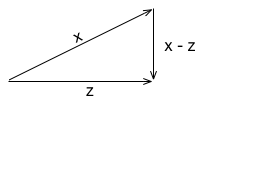
\includegraphics[width=50mm, scale=0.5]{x-minus-z.png}
\end{center}

The resulting transformation back to the original space, $\mathbf{v}^t = W\mathbf{z}^t$, loses no more information from the lower dimensional subspace and, hence, $|| \mathbf{z}^t || =|| \mathbf{v}^t ||$.

Given the previous information, that no information is lost in translating from the lower dimensional space to the original space, we can depict the figure above thus:

\begin{center}
  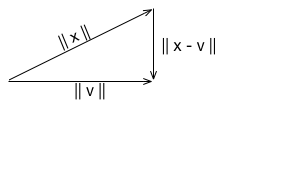
\includegraphics[width=50mm, scale=0.5]{x-minus-v.png}
\end{center}

So if we can prove that $ \mathbf{v}^t \perp (\mathbf{x}^t - \mathbf{v}^t)$, then by Pythagoras' theorem, we can prove the claim true.  The proof relies on the fact that for any two vectors that are orthogonal, their inner product is 0.  Therefore, we want to prove:

\begin{equation}
(\mathbf{x}^t - \mathbf{v}^t) \cdot \mathbf{v}^t = 0
\end{equation}

Given $\mathbf{v}^t = WW^T\mathbf{x}^t$, we replace $\mathbf{v}^t$ with $WW^T\mathbf{x}^t$:

\begin{equation}
\begin{aligned}
(\mathbf{x}^t - WW^T\mathbf{x}^t)(WW^T\mathbf{x}^t) &= 0 \\
\mathbf{x}^t WW^T \mathbf{x}^t - (WW^T\mathbf{x}^t)(WW^T\mathbf{x}^t) &= 0 \\
\mathbf{x}^t WW^T \mathbf{x}^t - (\mathbf{x}^tWW^T)(WW^T\mathbf{x}^t) &= 0 \\
\mathbf{x}^t WW^T \mathbf{x}^t - (\mathbf{x}^t(WW^TWW^T)\mathbf{x}^t) &= 0 \\
\mathbf{x}^t WW^T \mathbf{x}^t - (\mathbf{x}^t(W(W^TW)W^T)\mathbf{x}^t) &= 0 \\
\mathbf{x}^t WW^T \mathbf{x}^t - (\mathbf{x}^t(W(\mathbb{I})W^T)\mathbf{x}^t) &= 0 \\
\mathbf{x}^t WW^T \mathbf{x}^t - (\mathbf{x}^t(WW^T)\mathbf{x}^t) &= 0 \\
\mathbf{x}^t WW^T \mathbf{x}^t - \mathbf{x}^tWW^T\mathbf{x}^t &= 0 \\
0 &= 0
\end{aligned}
\end{equation}

Therefore:

\begin{equation}
(\mathbf{x}^t - \mathbf{v}^t) \cdot \mathbf{v}^t = 0
\end{equation}

The key to this proof is that $W^TW = \mathbb{I}$.  This is true because the matrix $W$ is assumed to contain the eigenvectors of $\mathbf{\Sigma}$ that are associated with unique eigenvalues.  Therefore the columns of $W$ are orthonormal and so $W^TW = \mathbb{I}$.

Because $  \mathbf{v}^t \perp (\mathbf{x}^t - \mathbf{v}^t) $, then the following holds by Pythagoras' theorem:

\begin{equation}
|| \mathbf{x}^t ||_2^2 = || \mathbf{v}^t ||_2^2 + || \mathbf{x} - \mathbf{v} ||_2^2
\end{equation}

Rearranging which gives:

\begin{equation}
|| \mathbf{x}^t ||_2^2 - || \mathbf{v}^t ||_2^2 = || \mathbf{x} - \mathbf{v} ||_2^2
\end{equation}

This is the solution for any vector $\mathbf{x}^t$, but holds for:

\begin{equation}
\sum\limits_{t=1}^N || \mathbf{x}^t ||_2^2 - \sum\limits_{t=1}^N || \mathbf{v}^t ||_2^2 = \sum\limits_{t=1}^N || \mathbf{x}^t - \mathbf{v}^t ||_2^2
\end{equation}

Since if this is true for any projection, it is true for all projections and the sums are trivial. Thus, the claim is proved true.

\section{Problem 2}

%2a
\subsection{(a) Show that the stochastic gradient descent update for $v_{i,h}$ is of the form $v_{i,h}^{new} = v_{i,h}^{old} + \Delta v_{i,h}$ with the update $\Delta v_{i,h} = \eta \Delta_i^t z_h^t$, where $\Delta_i^t = -g^{'}(a_i^t) \frac{ \partial L(r_i^t, y_i^t) }{ \partial y_i^t }$.}

The gradient descent update rule for $\Delta v_{i,h}$ has the form:

\begin{equation}
\Delta v_{i,h} = - \eta \frac{\partial E}{\partial v_{i,h} }
\end{equation}

Noting that we only need to update one weight, $v_{i,h}$, and that we are using stochastic gradient descent, we can remove the summations over $k$ and $N$ respectively, and rewrite the loss function that we need to evaluate as:

\begin{equation}
\begin{aligned}
E(W, V|Z) &= L(r_i^t, y_i^t) \\
&= L(r_i^t, g(a_i^t)) \\
&= L(r_i^t, g( \sum\limits_{h=1}^H v_{i,h} z_h^t +v_{i0}))
\end{aligned}
\end{equation}

According Alpaydin, the chain rule we need to evaluate is:

\begin{equation}
\frac{\partial E}{\partial v_{i,h}} = \frac{\partial E} {\partial y_i^t} \frac{\partial y_i^t} {\partial v_{i,h}}
\end{equation}

But, since we have an activation function, $g ( a_i^t )$, we will account for that with:

\begin{equation}
\frac{\partial E}{\partial v_{i,h}} = \frac{\partial E} {\partial y_i^t} \frac{\partial y_i^t} {\partial a_i^t} \frac{ \partial a_i^t }{\partial v_{i,h}}
\end{equation}

Applying the chain rule:

\begin{equation}
\begin{aligned}
\frac{\partial E}{\partial y_i^t} &= \frac{\partial L (r_i^t, y_i^t)}{\partial y_i^t} \\
\frac{\partial y_i^t}{\partial a_i^t} &= g^{'}(a_i^t) \\
\frac{ \partial a_i^t }{\partial v_{i,h}} &= \frac{ \partial }{\partial v_{i,h}} ( \sum\limits_{h=1}^H v_{i,h} z_h^t +v_{i0} ) = z_h^t
\end{aligned}
\end{equation}

Then the update rule is learning rate ($\eta$) $\times$ error ($\Delta_i^t$) $\times$ input ($z_h^t$):

\begin{equation}
\Delta v_{i,h} = \eta \Delta_i^t z_h^t
\end{equation}

Where the error $\Delta_i^t$ is:

\begin{equation}
\Delta_i^t = - g^{'}(a_i^t) \frac{ \partial L(r_i^t, y_i^t) }{ \partial y_i^t }
\end{equation}


% 2b
\subsection{(b) Show that the stochastic gradient descent update for $w_{h,j}$ is of the form $w_{h,j}^{new} = w_{h,j}^{old} + \Delta w_{h,j}$ with the update $\Delta w_{h,j} = \eta \Delta_h^t x_j^t$, where $\Delta_h^t = g^{'}(a_h^t) \sum_{i=1}^k \Delta_i^t v_{i,h}$ }

According to Alpaydin, the update rule for $w_{h,j}$ is:

\begin{equation}
\frac{ \partial E }{ \partial w_{h,j} } = \frac{\partial E}{\partial y_i} \frac{\partial y_i}{\partial z_h} \frac{\partial z_h}{\partial w_{h,j}}
\end{equation}

But, this time we have two activation functions, $g ( a_i^t )$ and $g ( a_h^t )$, for which we need to account:

\begin{equation}
\frac{ \partial E }{ \partial w_{h,j} } = \frac{ \partial E }{ \partial y_i^t }  \frac{ \partial y_i^t }{ \partial a_i^t }  \frac{ a_i^t }{ z_h }  \frac{ \partial z_h }{ \partial a_h^t }  \frac{ \partial a_h^t }{ \partial w_{h,j} }
\end{equation}

The error from the hidden layer to the output layer is propagated to this layer.  We see this in the terms:

\begin{equation}
\Delta_i^t = \frac{ \partial E }{ \partial y_i^t }  \frac{ \partial y_i^t }{ \partial a_i^t }
\end{equation}

We also need the partial derivative of $a_i^t$ with respect to $z_h$:

\begin{equation}
\frac{\partial}{z_h} ( \sum\limits_{h=1}^H v_{i,h} z_h^t + v_{i0} ) = v_{i,h}
\end{equation}

If there are $k$ output nodes, there are also $k$ weights ($v_{i,h}$) and the error for each of them has to be accounted for.  We account for that with:

\begin{equation}
\sum_{i=1}^k \Delta_i^t v_{i,h}
\end{equation}

And finishing off rest of the terms in the chain rule:

\begin{equation}
\begin{aligned}
\frac{\partial z_h} { \partial a_h^t } &= g^{'}(a_h^t) \\
\frac{ \partial a_h^t }{ \partial w_{h,j} } &= \frac{ \partial } { w_{h,j} } ( \sum\limits_{j=1}^d w_{h,j} x_j^t + w_0 ) = x_j^t
\end{aligned}
\end{equation}

Then the update rule is learning rate ($\eta$) $\times$ error ($\Delta_h^t$) $\times$ input ($x_j^t$):

\begin{equation}
\Delta w_{h,j} = \eta \Delta_h^t x_j^t
\end{equation}

Where the error $\Delta_h^t$ is:

\begin{equation}
\Delta_h^t = g^{'}(a_h^t) \sum_{i=1}^k \Delta_i^t v_{i,h}
\end{equation}

% 3

\section{Problem 3}

\subsection{Description}

MyFLDA2 is an implementation of Fisher's Linear Discriminant Analysis for two classes.  This implementation is run against the scikit-learn standard dataset Boston housing prices with changes as described below.  When the test file, $\textbf{q3.py}$, is run, a threshold is found for MyFLDA2 to predict from a given unseen observation from the data that minimizes training set error.  This can take a bit to run, but there is ample feedback so that a user will know this is happening.  The algorithm exhaustively runs 5-fold cross-validation against every observation in the dataset and one more for the average of the class means, and chooses a threshold for the model based on which threshold gives the lowest mean training set error.  This model with that threshold set is then run against the Boston50 and Boston75 datasets a final time to report the errors.  A sample run of this is documented below in the $\textbf{Results}$ section.

\subsection{Boston50 Housing Dataset}

The standard Boston housing prices dataset is used.  This dataset consists of 506 samples and 13 features.  It is typically used for regression, but we modify it for use in classification contexts.  The target data is split such that the lowest 50\% of the data is labeled -1 and the highest 50\% is labeled 1.  No other modifications are made to the dataset.

\subsection{Boston75 Housing Dataset}

The standard Boston housing prices dataset is used.  This dataset consists of 506 samples and 13 features.  It is typically used for regression, but we modify it for use in classification contexts.  The target data is split such that the lowest 75\% of the data is labeled -1 and the highest 25\% is labeled 1.  No other modifications are made to the dataset.

\subsection{Results}

\noindent method: MyFLDA2

\noindent dataset: Boston50

\begin{center}
	\begin{tabular}  { | l | l | l | l | l | l | l | }
	\hline
	Fold 1 & Fold 2 & Fold 3 & Fold 4 & Fold 5 & mean & std dev\\ \hline
	0.1275 & 0.1089 & 0.1980 & 0.1584 & 0.1386 & 0.1463 & 0.0304\\
	\hline
	\end{tabular}
\end{center}
\noindent method: MyFLDA2

\noindent dataset: Boston75

\begin{center}
	\begin{tabular}  { | l | l | l | l | l | l | l | }
	\hline
	Fold 1 & Fold 2 & Fold 3 & Fold 4 & Fold 5 & mean & std dev\\ \hline
	0.0588 & 0.1188 & 0.1287 & 0.1089 & 0.1188 & 0.1068 & 0.0248\\
	\hline
	\end{tabular}
\end{center}
\noindent method: LogisticRegression

\noindent dataset: Boston50

\begin{center}
	\begin{tabular}  { | l | l | l | l | l | l | l | }
	\hline
	Fold 1 & Fold 2 & Fold 3 & Fold 4 & Fold 5 & mean & std dev\\ \hline
	0.0784 & 0.2079 & 0.1188 & 0.1683 & 0.1089 & 0.1365 & 0.0460\\
	\hline
	\end{tabular}
\end{center}
\noindent method: LogisticRegression

\noindent dataset: Boston75

\begin{center}
	\begin{tabular}  { | l | l | l | l | l | l | l | }
	\hline
	Fold 1 & Fold 2 & Fold 3 & Fold 4 & Fold 5 & mean & std dev\\ \hline
	0.0784 & 0.1287 & 0.1188 & 0.0891 & 0.0693 & 0.0969 & 0.0230\\
	\hline
	\end{tabular}
\end{center}


% Extra Credit

\section{Extra Credit}

\subsection{Is $L_{sq}^{(tlu)}(\mathbf{w})$ a convex function of the parameter $\mathbf{w}$?}

No, $L_{sq}^{(tlu)}$ is $\textbf{not}$ a convex function.  If we assume our function is in $\mathbb{R}^2$ and $y=1$ and look at the plot of the function $(1 - ( max(0, a) + 0.5 min(0, a)))^2$:


\begin{center}
  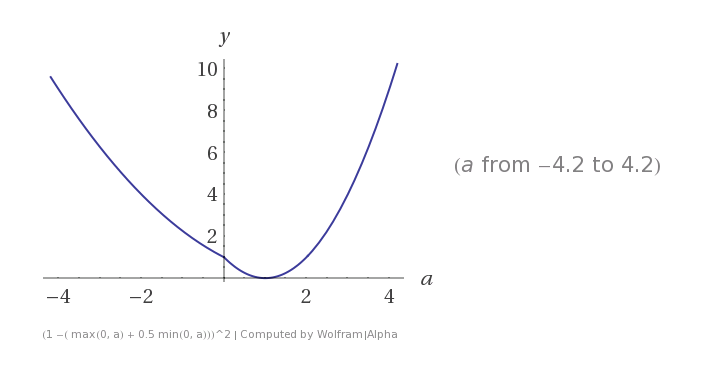
\includegraphics[width=50mm, scale=0.5]{plot1.png}
\end{center}

We see a little "kink" at $(0, 1)$.  Given this definition of convexity:

\begin{equation}
f ( t\mathbf{x}_1 + (1 - t)\mathbf{x}_2) \leq tf ( \mathbf{x}_1) + (1 - t)f(\mathbf{x}_2)
\end{equation}

If we let:

\begin{equation}
\begin{aligned}
x_1 &= -0.04 \\
x_2 &= 0.04 \\
w &= 1.0 \\
t &= 0.9
\end{aligned}
\end{equation}

We will show that this function is not convex.  Noticing that $\mathbf{w}$ is a scalar and set to 1, we ignore it.  The function we need to evaluate in our definition of convexity, given by $f(x)$ is:
\begin{equation}
f(x) = (1 - (max(0, x) + 0.5 min(0, x)))^2
\end{equation}

\begin{equation}
\begin{aligned}
t\mathbf{x}_1 + (1 - t)\mathbf{x}_2 &= (0.9)(-0.04) + (1 - 0.9)0.04 = -0.032 \\
f(-0.032) = (1 - (max(0, -0.032) + 0.5 min(0, -0.032)))^2 &= \textbf{1.032256} \\
f(\mathbf{x}_1) = (1 - (max(0, -0.04) + 0.5 min(0, -0.04)))^2 &= 1.0404 \\
f(\mathbf{x}_2) = (1 - (max(0, 0.04) + 0.5 min(0, 0.04)))^2 &= 0.9216 \\
tf(\mathbf{x}_1) + (1 - t)f(\mathbf{x}_2) = (0.9)(1.0404) + (1 - 0.9)(0.9216) &= \textbf{1.02852} \\
\textbf{1.032256} &\leq \textbf{1.02852} == False
\end{aligned}
\end{equation}

Therefore we conclude that the function is $\textbf{not}$ convex.

\end{document}
